% arXiv submission draft (LoCoMo Dialog RAG / Entity--Memory)
% Compile: pdflatex main && bibtex main && pdflatex main && pdflatex main
% Or upload this folder to Overleaf.
\documentclass[11pt]{article}

\usepackage[margin=1in]{geometry}
\usepackage{times}
\usepackage{latexsym}
\usepackage{amsmath,amssymb,amsfonts}
\usepackage{booktabs}
\usepackage{multirow}
\usepackage{graphicx}
\usepackage{xcolor}
\usepackage{natbib}
\usepackage{hyperref}
\usepackage{url}
\usepackage{enumitem}
\usepackage{array}
\usepackage{tabularx}
\usepackage{caption}
\usepackage{subcaption}
\usepackage{algorithm}
\usepackage{algpseudocode}
\usepackage{tikz}
\usetikzlibrary{positioning,arrows.meta}
\usepackage[T1]{fontenc}
\usepackage[utf8]{inputenc}

\hypersetup{
  colorlinks=true,
  linkcolor=blue!50!black,
  citecolor=blue!50!black,
  urlcolor=blue!50!black
}

\title{Entity--Memory Bipartite Graphs for\\Long-Conversation Dialog Retrieval on LoCoMo}
\author{
  Anonymous Authors
  % Fill real names/affiliations for a named arXiv upload.
}
\date{}

\begin{document}
\maketitle

\begin{abstract}
Long multi-session conversations require retrieval that is both semantically flexible and entity-grounded.
We study a conversation-only \textbf{Entity--Memory (EM)} bipartite graph for LoCoMo \textbf{long-term conversational QA}.
Each dialog turn is a Memory node; LLM-extracted entities are Entity nodes linked by Mentions; consecutive turns are linked by dialog-order sequence edges.
At query time we soft-match question entities to graph entities with BM25, optionally expand $\pm 1$ neighbors along the dialog sequence, score the gated Memory pool with dense embeddings, and fuse the two signals as $0.30\cdot E + 0.70\cdot S$.

To isolate the contribution of this retrieval structure, we rebuild the pipeline under a \textbf{matched stack}: entity extraction and answering with \texttt{gpt-3.5-turbo}, embeddings with \texttt{text-embedding-3-small}, and the LoCoMo short-answer protocol (token-F1 and evidence recall).
On LoCoMo-10 (10 conversations, 1986 QA items), EM fusion retrieval (System~B) reaches \textbf{46.48} token-F1@25 and \textbf{82.54\%} recall\_acc@25, improving over a plain full-corpus Dialog embedding RAG baseline (System~A: 44.99 F1, 78.53\% recall) by \textbf{+1.49} F1 points and \textbf{+4.01} recall points.
Ablations show that entity-only ranking is insufficient (40.78 F1), embedding-only on the same Memory corpus nearly matches A (44.83 F1), and disabling sequence expansion yields a small drop (46.20 F1 / 80.77\% recall).
We cite LoCoMo Table~3 Dialog/Observation numbers only as external anchors, because the original paper uses a different retriever (DRAGON).
\end{abstract}

\section{Introduction}
\label{sec:intro}

LoCoMo~\citep{maharana2024locomo} evaluates long-term conversational memory with multi-session dialogs and category-stratified QA (multi-hop, temporal, open-domain, single-hop, adversarial).
In the paper's RAG comparison, systems retrieve a unit of memory---raw dialog turns, speaker observations, or session summaries---and a reader produces a short answer.
Official metrics are \textbf{token-level F1} of the answer and \textbf{retrieval recall} of gold evidence dialog IDs at cutoffs $k$.

This paper stays inside the \textbf{Dialog-family} setting: the system must retrieve dialog turns and answer from those turns.
The question is whether an \textbf{entity-aware graph over conversation turns} improves Dialog retrieval when confounding factors are controlled.

\paragraph{Matched-stack requirement.}
A high F1 can come from a stronger embedder, a stronger reader, a different prompt, or leakage of QA annotations into the memory store.
Our primary comparison is therefore:

\begin{quote}
\textit{System A vs.\ System B under the same embedding model, the same answer model, the same answer prompt, the same dataset split, and the same metrics.
Entity extraction (when used) also uses the same LLM.}
\end{quote}

LoCoMo Table~3 numbers (Dialog F1@25~$=$~41.0, Dialog R@25~$=$~76.7, Observation best F1~$=$~43.3) appear only as \textbf{external citations}.
They use DRAGON retrieval; we use \texttt{text-embedding-3-small}.
Sharing the reader (\texttt{gpt-3.5-turbo}) does \emph{not} make the paper comparison a matched-retriever experiment.

\paragraph{Contributions.}
\begin{enumerate}[leftmargin=*,itemsep=2pt]
  \item A conversation-only Entity--Memory bipartite construction with Mentions and dialog-order Memory sequence edges, excluding QA fields from graph construction.
  \item A retrieval procedure that combines BM25 entity soft-match gating, optional $\pm 1$ sequence expansion, and dense Memory scoring with fixed fusion weights $0.30/0.70$.
  \item A matched-stack LoCoMo-10 evaluation: plain Dialog dense RAG (A) vs.\ EM fusion (B), plus entity-only / embed-only / no-sequence ablations, with hyperparameters fully specified.
\end{enumerate}

\section{Related Work}
\label{sec:related}

\paragraph{LoCoMo.}
\cite{maharana2024locomo} introduce long multi-session conversations and evaluate long-context models and RAG variants (Dialog / Observation / Summary).
Official QA metrics are token F1 and evidence recall; the RAG tables we cite use DRAGON~+~GPT-3.5.

\paragraph{Retrieval-augmented generation.}
RAG~\citep{lewis2020rag} and dense passage retrieval~\citep{karpukhin2020dpr} retrieve text units for a reader.
We retrieve \emph{dialog turns} and keep the LoCoMo short-answer reader fixed while changing only the retrieval structure.

\paragraph{Lexical and dense signals.}
BM25~\citep{robertson2009bm25} remains a strong lexical baseline; we use it for short entity-key soft-match, not as the sole Memory ranker.
Dense embeddings~\citep{openai2023embeddings} provide semantic ranking over Memory text.

We intentionally omit industrial LLM-as-judge protocols from the main tables; those scores measure a different evaluation contract than LoCoMo's official F1/recall.

\section{Method}
\label{sec:method}

Figure~\ref{fig:overview} summarizes the pipeline: conversation-only graph construction, query-time entity soft-match with optional sequence expansion, dense scoring on the candidate pool, fusion ranking, and short-answer generation.

\begin{figure}[t]
\centering
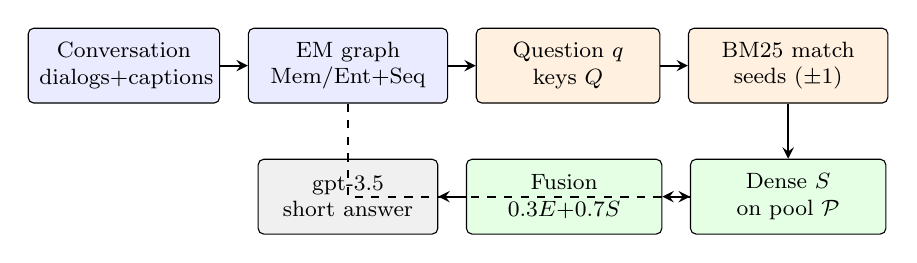
\begin{tikzpicture}[
  font=\footnotesize,
  box/.style={draw, rounded corners=2pt, align=center, inner sep=4pt, minimum height=0.95cm},
  arr/.style={->, thick, >=stealth}
]
  \node[box, fill=blue!8, text width=2.15cm] (conv) {Conversation\\dialogs+captions};
  \node[box, fill=blue!8, text width=2.25cm, right=0.35cm of conv] (graph) {EM graph\\Mem/Ent+Seq};
  \node[box, fill=orange!12, text width=2.05cm, right=0.35cm of graph] (q) {Question $q$\\keys $Q$};
  \node[box, fill=orange!12, text width=2.25cm, right=0.35cm of q] (gate) {BM25 match\\seeds ($\pm1$)};
  \node[box, fill=green!10, text width=2.2cm, below=0.7cm of gate] (dense) {Dense $S$\\on pool $\mathcal{P}$};
  \node[box, fill=green!10, text width=2.2cm, left=0.35cm of dense] (fuse) {Fusion\\$0.3E{+}0.7S$};
  \node[box, fill=gray!12, text width=2.0cm, left=0.35cm of fuse] (ans) {gpt-3.5\\short answer};
  \draw[arr] (conv) -- (graph);
  \draw[arr] (graph) -- (q);
  \draw[arr] (q) -- (gate);
  \draw[arr] (gate) -- (dense);
  \draw[arr] (dense) -- (fuse);
  \draw[arr] (fuse) -- (ans);
  \draw[arr, dashed] (graph.south) |- (dense.west);
\end{tikzpicture}
\caption{Overview of Entity--Memory Dialog retrieval (System~B).
Solid arrows: query-time path; dashed arrow: Memory embeddings come from the conversation graph.}
\label{fig:overview}
\end{figure}

\subsection{Conversation-only inputs}
\label{sec:inputs}

For each LoCoMo sample, graph construction may use session dialogs with fields in Table~\ref{tab:fields}.
QA questions, gold answers, gold evidence, category labels, judge outputs, and previous predictions are \textbf{forbidden} at graph construction.
Question-side entity extraction runs at query time and does not write into the stored graph.

\begin{table}[t]
\centering
\small
\caption{Fields used when building the conversation graph.}
\label{tab:fields}
\begin{tabular}{llp{6.2cm}}
\toprule
Field & In graph? & Role \\
\midrule
\texttt{dia\_id} & yes & Memory identity; retrieval returns these IDs \\
\texttt{speaker} & yes & Attribute; pronoun replacement; embedding text \\
\texttt{text} & yes & Raw utterance on Memory \\
\texttt{blip\_caption}/\texttt{img\_caption} & yes & Optional image caption on Memory \\
\texttt{session\_*\_date\_time} & yes & Timestamp on Memory; answer context; temporal QA \\
QA question/answer/evidence/category & \textbf{no} & Evaluation / query time only \\
\bottomrule
\end{tabular}
\end{table}

\subsection{Preprocessing}
\label{sec:prep}

Each dialog text is normalized with \texttt{replace\_pronouns(text, speaker, previous\_speaker, dialog\_time)}:
first-person pronouns map to the current speaker; second-person pronouns map to the previous speaker when available; relative time expressions may resolve against the session date string.
Each Memory stores both raw \texttt{text} and \texttt{text\_normalized}.
Entity extraction runs on the normalized dialog string (and caption text when included by the builder).

\subsection{Graph schema}
\label{sec:schema}

\paragraph{Memory node $m$.}
One per dialog turn, with identity \texttt{memory:\{dia\_id\}}, plus session index, \texttt{date\_time}, speaker, raw/normalized text, and optional caption.

\paragraph{Entity node $e$.}
LLM-extracted concept with type in
$\{\texttt{Who},\texttt{What},\texttt{When},\texttt{Where},\texttt{Why},\texttt{How},\texttt{How much}\}$,
canonicalized by a string key normalizer.

\paragraph{Edges.}
(1)~\textbf{Mentions} between Entity and Memory when an entity is extracted from that turn.
(2)~\textbf{Sequence}: bidirectional \texttt{NEXT}/\texttt{PREV} between consecutive Memories in conversation order.
Mentions are bipartite Entity--Memory; sequence edges are Memory--Memory.

\subsection{Entity extraction (v4)}
\label{sec:extract}

We use extract version \texttt{v4} with \texttt{gpt-3.5-turbo}.
The fixed prompt (scaffold length 2430 characters) asks for high-signal short noun phrases, encourages subject--predicate--object coverage when present, forbids interrogatives/function words and generic auxiliaries, and requests a JSON array of \texttt{\{"value","type"\}}.
Extraction chat uses temperature $0.3$ and a 2500-token budget (non-\texttt{gpt-5} models), with up to three parse retries.
The same extractor produces question entity keys $Q$ at query time (cached per sample; not stored in the conversation graph).
The builder also attaches the speaker as an entity when \texttt{add\_speaker\_as\_entity=True} (package default).

\subsection{Dense Memory index}
\label{sec:embed}

The embedding string for Memory $m$ is the concatenation of
\texttt{text\_normalized}, \texttt{text}, \texttt{speaker}, \texttt{blip\_caption}, and \texttt{query}.
We embed with \texttt{text-embedding-3-small} and score by cosine similarity against the question embedding (non-positive similarities clipped at 0 in the score map).
In the evaluation runner, shared cross-model text caches are disabled to avoid mixing embedding dimensionalities; per-sample \texttt{.npz} caches are used.

\subsection{Entity BM25 soft-match}
\label{sec:bm25}

We build a BM25Okapi index over Entity documents (\texttt{key}/\texttt{value} tokens).
For each question key $q_k\in Q$:
(1)~score all entities and peak-normalize to $[0,1]$;
(2)~force exact normalized key matches to score $1.0$;
(3)~keep entities with score $\ge 0.5$, at most 20 entities per question key.

\subsection{Entity$\rightarrow$Memory scores and sequence expansion}
\label{sec:seeds}

Matched entities receive strength
\begin{equation}
\mathrm{raw}(e)=\left(\frac{\sum_{q_k}\mathrm{match}(e,q_k)}{|Q_{\mathrm{eff}}|}\right)\cdot\frac{1}{\log(1+\deg(e))},
\end{equation}
where $Q_{\mathrm{eff}}$ is the set of question keys that matched at least one entity and $\deg(e)$ is the Mentions degree.
Scores propagate over Mentions to Memories.
Who-like and content matches are tracked separately: if content score $c>0$, the seed is $\max(c,w)$; if only Who scores exist, dampen by $0.25$ ($E_{\mathrm{seed}}(m)=0.25\cdot w$).

If sequence expansion is enabled, each dialog-order neighbor $n$ of a seed with score $s>0$ receives
$E(n)\leftarrow\max(E(n),\,0.5\cdot s)$
(one hop).

\subsection{Fusion ranking}
\label{sec:fusion}

Let $E(m)$ be the (possibly expanded) entity score and $S(m)$ the dense score.
If the entity map is non-empty, the candidate pool $\mathcal{P}$ is its support and dense scores are computed only on $\mathcal{P}$; otherwise $\mathcal{P}$ is the full Memory corpus.
Final score:
\begin{equation}
\mathrm{score}(m)=0.30\cdot E(m)+0.70\cdot S(m).
\end{equation}
Return top-$k$ dialog IDs by descending score (tie-break by \texttt{dia\_id}).

Algorithm~\ref{alg:b} summarizes System~B.

\begin{algorithm}[t]
\caption{EM fusion retrieval (System B)}
\label{alg:b}
\begin{algorithmic}[1]
\Require graph $G$, question $q$, cutoff $k$
\State $Q \gets \mathrm{ExtractEntityKeys}(q)$ \Comment{\texttt{gpt-3.5-turbo}, v4}
\If{$Q \neq \emptyset$}
  \State $M \gets \mathrm{BM25SoftMatch}(G,Q;\ \mathrm{min\_rel}{=}0.5,\ \mathrm{top}{=}20)$
  \State $E \gets \mathrm{PropagateMentions}(G,M)$ \Comment{Who dampen $0.25$}
  \State $E \gets \mathrm{ExpandNeighbors}(E,\ \mathrm{scale}{=}0.5)$ \Comment{optional}
\Else
  \State $E \gets \emptyset$
\EndIf
\If{$E \neq \emptyset$}
  \State $\mathcal{P} \gets \mathrm{keys}(E)$;\; $S \gets \mathrm{EmbedScores}(q,\mathcal{P})$
\Else
  \State $\mathcal{P} \gets \mathrm{AllMemories}(G)$;\; $S \gets \mathrm{EmbedScores}(q,\mathcal{P})$
\EndIf
\ForAll{$m \in \mathcal{P}$}
  \State $\mathrm{score}(m) \gets 0.30\,E(m)+0.70\,S(m)$
\EndFor
\State \Return top-$k$ \texttt{dia\_id} by $\mathrm{score}$
\end{algorithmic}
\end{algorithm}

\subsection{Illustrative retrieval walk-through}
\label{sec:case}

Figure~\ref{fig:case} sketches a typical query-time path (schematic; not a cherry-picked benchmark win).
Suppose the question is \emph{``When did Caroline attend the support group?''}.
Extract-v4 yields keys such as \texttt{caroline} (Who) and \texttt{support group} (What).
BM25 soft-match links these keys to Entity nodes that Mentions-connect to dialog Memories near the relevant session (seed turns).
Sequence expansion then adds the immediate previous/next turns at half entity weight, which often carry dates or clarifications adjacent to the entity mention.
Dense scoring re-ranks the resulting pool with the question embedding; fusion ($0.30/0.70$) prefers turns that are both entity-linked and semantically aligned.
The top-25 dialogs are concatenated for the short reader.
In contrast, System~A scores \emph{all} turns by embedding alone and never forms an entity-conditioned pool.

\begin{figure}[t]
\centering
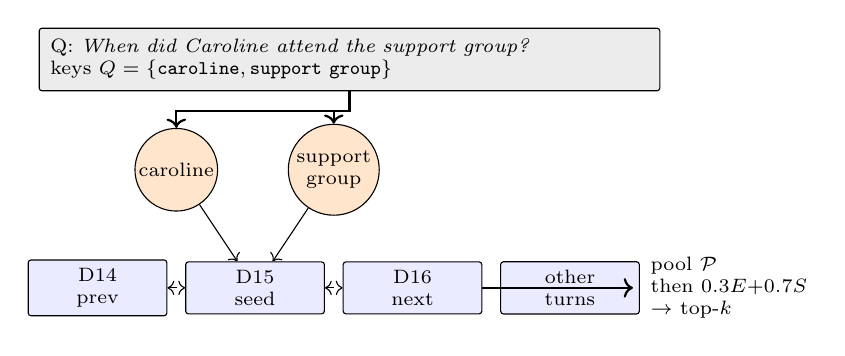
\begin{tikzpicture}[
  font=\scriptsize,
  m/.style={draw, rounded corners=1pt, fill=blue!8, align=center, inner sep=3pt, text width=1.55cm},
  e/.style={draw, circle, fill=orange!20, inner sep=1pt, minimum size=0.85cm, align=center},
  q/.style={draw, rounded corners=1pt, fill=gray!15, align=left, inner sep=4pt, text width=7.6cm}
]
  \node[q] (qq) at (0,2.6) {Q: \emph{When did Caroline attend the support group?}\\
  keys $Q=\{\texttt{caroline},\texttt{support group}\}$};
  \node[e] (e1) at (-2.2,1.2) {caroline};
  \node[e] (e2) at (-0.2,1.2) {support\\group};
  \node[m] (m1) at (-3.2,-0.3) {D14\\prev};
  \node[m] (m2) at (-1.2,-0.3) {D15\\seed};
  \node[m] (m3) at (0.8,-0.3) {D16\\next};
  \node[m] (m4) at (2.8,-0.3) {other\\turns};
  \draw[->,thick] (qq.south) -- ++(0,-0.25) -| (e1);
  \draw[->,thick] (qq.south) -- ++(0,-0.25) -| (e2);
  \draw[->] (e1) -- (m2);
  \draw[->] (e2) -- (m2);
  \draw[<->,dashed] (m1) -- (m2);
  \draw[<->,dashed] (m2) -- (m3);
  \node[anchor=west,align=left] at (3.7,-0.3) {pool $\mathcal{P}$\\then $0.3E{+}0.7S$\\$\rightarrow$ top-$k$};
  \draw[->,thick] (m3.east) -- (3.6,-0.3);
\end{tikzpicture}
\caption{Schematic retrieval case: question keys soft-match to entities, Mentions select seed Memories, $\pm 1$ sequence edges expand the pool, and fusion ranks dialogs for the reader.
Gray ``other turns'' remain outside the gated pool unless entity match fails and the system falls back to full-corpus dense retrieval.}
\label{fig:case}
\end{figure}

\subsection{Answer generation}
\label{sec:answer}

Top-25 retrieved dialogs form the context as
\begin{center}
\small\texttt{\{date\_time\}: \{speaker\} said, "\{text\}"[ and shared \{caption\}]}
\end{center}
in retrieval order.
The reader is \texttt{gpt-3.5-turbo} with temperature $0$ and default 512 completion tokens (retry with larger budgets on empty outputs).

\paragraph{Default prompt (category $\neq 5$).}
\textit{Based on the above context, write an answer in the form of a short phrase for the following question. Answer with exact words from the context whenever possible.}\\
\textit{Question: \{q\} Short answer:}

\paragraph{Temporal (category $=2$).}
Append ``Use DATE of CONVERSATION to answer with an approximate date.'' to the question before the template.

\paragraph{Adversarial (category $=5$).}
\textit{If the answer is not mentioned in the conversation, reply exactly: Not mentioned in the conversation.}

\subsection{Metrics}
\label{sec:metrics}

\paragraph{Token-F1.}
Lowercase alphanumeric tokens.
With gold/pred token sets $G,P$: both empty $\rightarrow 1$; either empty $\rightarrow 0$; else standard set F1.
We report mean $\times 100$ at answer cutoff $k{=}25$, plus diagnostic ex-category-5 means.

\paragraph{recall\_acc@$k$.}
For gold evidence ID list $E$ and retrieved list $R_k$,
$\lvert\{e\in E:e\in R_k\}\rvert/\lvert E\rvert$
(empty $E\rightarrow 1$).
Hit@$k$ is $1$ iff $E\cap R_k\neq\emptyset$.

Category IDs: 1 multi-hop, 2 temporal, 3 open-domain, 4 single-hop, 5 adversarial.
Overall includes category~5 unless labeled ex-cat5.

\section{Experimental Setup}
\label{sec:setup}

\subsection{Dataset and environment}

We evaluate all QA items with non-empty questions in \texttt{locomo10.json}: \textbf{1986} items over 10 conversations
(\texttt{conv-26,30,41,42,43,44,47,48,49,50}).

Matched stack:
\begin{itemize}[leftmargin=*,itemsep=1pt]
  \item Extract / answer: \texttt{gpt-3.5-turbo}
  \item Embeddings: \texttt{text-embedding-3-small}
  \item Fusion (B): $w_E{=}0.30$, $w_S{=}0.70$, sequence on
  \item Answer cutoff: top-25; recall sheet also uses $k\in\{5,10,25,50\}$
  \item Parallel answer workers: 8; embedding wait $0.05$s between batches in our runner
\end{itemize}

Graph statistics under gpt-3.5 extract-v4 are in Table~\ref{tab:graphs}.

\begin{table}[t]
\centering
\small
\caption{EM graph sizes after gpt-3.5 extract-v4 (matched stack).}
\label{tab:graphs}
\begin{tabular}{lrrrr}
\toprule
Sample & Mem. & Ent. & Mentions & Seq.\ edges \\
\midrule
conv-26 & 419 & 1120 & 2765 & 836 \\
conv-30 & 369 & 784 & 2151 & 736 \\
conv-41 & 663 & 1487 & 4204 & 1324 \\
conv-42 & 629 & 1255 & 3335 & 1256 \\
conv-43 & 680 & 1534 & 4038 & 1358 \\
conv-44 & 675 & 1281 & 3786 & 1348 \\
conv-47 & 689 & 1521 & 3944 & 1376 \\
conv-48 & 681 & 1446 & 3786 & 1360 \\
conv-49 & 509 & 1079 & 2750 & 1016 \\
conv-50 & 568 & 1241 & 3643 & 1134 \\
\bottomrule
\end{tabular}
\end{table}

\subsection{Systems}
\label{sec:systems}

Table~\ref{tab:systems} lists exact retrieval knobs.
All systems share the reader and prompts in \S\ref{sec:answer}.

\begin{table}[t]
\centering
\small
\caption{Retrieval configurations. ``Full pool'' means all Memory nodes.}
\label{tab:systems}
\begin{tabular}{lccccc}
\toprule
ID & Graph & $w_E$ & $w_S$ & Seq. & Pool \\
\midrule
A & Memory-only & 0.0 & 1.0 & off & full \\
B & EM v4 & 0.30 & 0.70 & on & gated$^\dagger$ \\
B\_entity & EM v4 & 1.0 & 0.0 & on & gated$^\dagger$ \\
B\_embed & EM v4 & 0.0 & 1.0 & off & full$^\ddagger$ \\
B\_noseq & EM v4 & 0.30 & 0.70 & off & gated$^\dagger$ \\
\bottomrule
\multicolumn{6}{p{0.95\linewidth}}{\footnotesize $^\dagger$Entity-gated; fall back to full corpus if no entity scores.
$^\ddagger$Question entity keys forced empty so retrieval cannot use Mentions.}
\end{tabular}
\end{table}

\paragraph{System A.}
Builds a Memory-only graph from the same conversation fields (no LLM entity extract at build time) and ranks all Memories by embedding cosine.
This is the fair plain Dialog dense RAG baseline under \texttt{text-embedding-3-small}.

\paragraph{System B\_embed.}
Uses Memories from the EM graph but forces empty question keys, so ranking is full-corpus cosine---a dense-only control on the same Memory units as B.

\section{Results}
\label{sec:results}

\subsection{Main comparison}

Table~\ref{tab:main} reports overall metrics.
Under the matched stack, System~B improves both primary metrics over A
($\Delta$F1~$=+1.49$, $\Delta$recall@$25$~$=+4.01$).
We treat joint improvement on token-F1@25 and recall\_acc@25 as evidence that the retrieval structure helps, rather than trading one metric for the other.

\begin{table}[t]
\centering
\small
\caption{Matched-stack LoCoMo-10 results ($n{=}1986$). F1 is token-F1@25 (\%). Recall/hit are \%.}
\label{tab:main}
\begin{tabular}{lrrrrrrr}
\toprule
System & F1 & ex5 F1 & R@25 & Hit@25 & R@5 & R@10 & R@50 \\
\midrule
A & 44.99 & 50.20 & 78.53 & 83.69 & 56.95 & 67.21 & 85.61 \\
\textbf{B} & \textbf{46.48} & \textbf{51.68} & \textbf{82.54} & \textbf{87.56} & \textbf{62.82} & \textbf{72.92} & \textbf{88.82} \\
B\_entity & 40.78 & 45.27 & 65.99 & 71.75 & 41.98 & 52.37 & 73.41 \\
B\_embed & 44.83 & 49.99 & 78.53 & 83.69 & 56.95 & 67.26 & 85.56 \\
B\_noseq & 46.20 & 51.05 & 80.77 & 85.95 & 60.70 & 70.62 & 86.72 \\
\bottomrule
\end{tabular}
\end{table}

\subsection{Category breakdown}

Table~\ref{tab:cat} reports $k{=}25$ by category for A and B.
Overall gains are driven especially by single-hop (F1 $60.69\rightarrow 63.22$; recall $87.22\rightarrow 90.61$) and adversarial recall ($71.75\rightarrow 81.73$); the LoCoMo \emph{open-domain} category (dataset category~3) also improves.
Multi-hop F1 is nearly flat while multi-hop recall\_acc slightly decreases; temporal F1 dips slightly while temporal recall rises.
These mixed per-category movements caution against claiming uniform gains on every category; we therefore emphasize overall F1 and overall recall together.

\begin{table}[t]
\centering
\small
\caption{Category results at $k{=}25$ (F1 \%, recall\_acc \%, hit \%).}
\label{tab:cat}
\begin{tabular}{llrrrr}
\toprule
Sys. & Category & $n$ & F1 & R@25 & Hit@25 \\
\midrule
\multirow{5}{*}{A}
 & Multi-hop & 282 & 38.73 & 60.96 & 86.52 \\
 & Temporal & 321 & 42.55 & 88.89 & 91.28 \\
 & Open-domain & 96 & 17.60 & 50.91 & 62.50 \\
 & Single-hop & 841 & 60.69 & 87.22 & 88.11 \\
 & Adversarial & 446 & 26.98 & 71.75 & 72.65 \\
\midrule
\multirow{5}{*}{B}
 & Multi-hop & 282 & 38.88 & 59.97 & 84.40 \\
 & Temporal & 321 & 42.17 & 90.19 & 92.52 \\
 & Open-domain & 96 & 20.05 & 56.42 & 68.75 \\
 & Single-hop & 841 & 63.22 & 90.61 & 91.44 \\
 & Adversarial & 446 & 28.53 & 81.73 & 82.74 \\
\bottomrule
\end{tabular}
\end{table}

\subsection{Ablation analysis}
\label{sec:ablation}

\paragraph{Entity-only (B\_entity).}
Removing dense scores collapses overall F1 to 40.78 and recall\_acc@25 to 65.99\%.
Entity soft-match can surface Mentions-linked turns, but without dense ranking it cannot order candidates by question paraphrase similarity.
Entities are a candidate/feature channel, not a complete ranker.

\paragraph{Embed-only (B\_embed).}
Forcing an empty entity key set yields full-corpus cosine on EM Memories: F1 44.83, recall\_acc@25 78.53\%, essentially matching A.
Storing entities on disk does nothing if unused in scoring; B's gain over A is not explained by ``using an EM file format.''

\paragraph{No sequence (B\_noseq).}
Disabling $\pm 1$ expansion yields F1 46.20 and recall\_acc@25 80.77\% ($\Delta$ vs.\ B: $-0.28$ F1, $-1.77$ recall).
Neighbors help when gold evidence is adjacent to an entity-matched turn, but most of the lift vs.\ A already appears from gated fusion without sequence.

\paragraph{Interpretation of ablations.}
These controls are best read as \textbf{hypothesis filters}, not as a strict causal identification of every mechanism.
They \emph{disfavor} several simple accounts of the A$\rightarrow$B gap:
(i)~if the gain were only packaging of Memory text, B\_embed would beat A substantially---it does not;
(ii)~if entities alone sufficed without dense semantics, B\_entity would approach B---it does not;
(iii)~if sequence edges explained most of the lift, B\_noseq would collapse toward A---it remains clearly above A.
A remaining account consistent with the pattern is \textbf{entity-conditioned candidate formation combined with dense ranking under $0.30/0.70$ fusion}, with sequence as a secondary term.
We do not claim that this is the unique causal pathway, nor that every category benefits for the same reason.
Figure~\ref{fig:ablation} visualizes token-F1@25 across variants.

\begin{figure}[t]
\centering
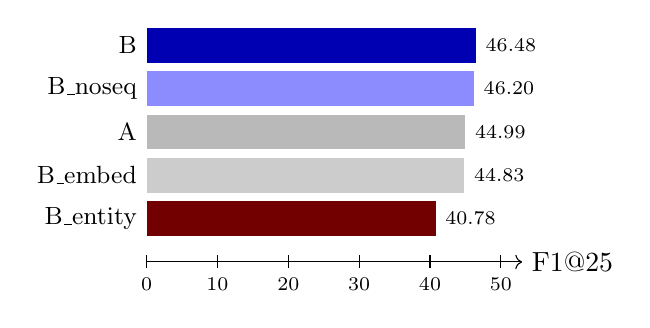
\begin{tikzpicture}[x=0.09cm,y=0.55cm]
  \def\xmax{50}
  \draw[->] (0,0) -- (\xmax+3,0) node[right] {F1@25};
  \foreach \x in {0,10,20,30,40,50}
    \draw (\x,0.15) -- (\x,-0.15) node[below,font=\scriptsize] {\x};
  % bars (values from Table~\ref{tab:main})
  \fill[blue!70!black] (0,4.6) rectangle (46.48,5.4);
  \node[left,font=\small] at (0,5) {B};
  \node[right,font=\scriptsize] at (46.48,5) {46.48};
  \fill[blue!45] (0,3.6) rectangle (46.20,4.4);
  \node[left,font=\small] at (0,4) {B\_noseq};
  \node[right,font=\scriptsize] at (46.20,4) {46.20};
  \fill[gray!55] (0,2.6) rectangle (44.99,3.4);
  \node[left,font=\small] at (0,3) {A};
  \node[right,font=\scriptsize] at (44.99,3) {44.99};
  \fill[gray!40] (0,1.6) rectangle (44.83,2.4);
  \node[left,font=\small] at (0,2) {B\_embed};
  \node[right,font=\scriptsize] at (44.83,2) {44.83};
  \fill[red!45!black] (0,0.6) rectangle (40.78,1.4);
  \node[left,font=\small] at (0,1) {B\_entity};
  \node[right,font=\scriptsize] at (40.78,1) {40.78};
\end{tikzpicture}
\caption{Ablation of token-F1@25 under the matched stack.
B and B\_noseq dominate; B\_embed$\approx$A; B\_entity collapses.}
\label{fig:ablation}
\end{figure}

\subsection{External citation of LoCoMo Table~3}

\begin{table}[t]
\centering
\small
\caption{External anchors from \cite{maharana2024locomo} vs.\ our matched stack.
Paper rows use DRAGON; ours use \texttt{text-embedding-3-small}. Not a matched-retriever comparison.}
\label{tab:paper}
\begin{tabular}{llrr}
\toprule
Source & Retriever & F1@25 & R@25 \\
\midrule
Paper Dialog & DRAGON & 41.0 & 76.7 \\
Paper Obs.\ (best F1) & DRAGON & 43.3 & -- \\
Our A & TES & 44.99 & 78.53 \\
Our B & TES & 46.48 & 82.54 \\
\bottomrule
\end{tabular}
\end{table}

Table~\ref{tab:paper} places our numbers next to paper Dialog/Observation anchors.
We do \textbf{not} treat $(B-\text{paper Dialog})$ as a controlled ablation of Entity--Memory vs.\ DRAGON.

\section{Limitations}
\label{sec:limits}

\begin{itemize}[leftmargin=*,itemsep=2pt]
  \item Retriever mismatch vs.\ the LoCoMo paper (DRAGON $\neq$ \texttt{text-embedding-3-small}).
  \item Entity quality depends on \texttt{gpt-3.5-turbo} extract-v4; stronger extractors may change absolutes.
  \item Multi-hop recall does not improve with B; error analysis remains open.
  \item No long-context no-retrieval ceiling (LoCoMo Table~2 style) in this draft.
  \item English-only pronoun/time heuristics; single benchmark (LoCoMo-10).
  \item LLM-as-judge / industrial memory scores are out of scope for the main table.
\end{itemize}

\section{Conclusion}
\label{sec:conclusion}

Under a fixed stack---\texttt{gpt-3.5-turbo} extract-v4, \texttt{text-embedding-3-small}, and \texttt{gpt-3.5-turbo} LoCoMo short answering---Entity--Memory fusion retrieval with weights $0.30/0.70$ and $\pm 1$ sequence expansion improves both token-F1@25 and evidence recall\_acc@25 over plain Dialog embedding RAG on LoCoMo-10.
Ablations \emph{exclude} several alternative explanations (dense packaging alone; entity scores alone; sequence-dominant gains) and are consistent with entity-conditioned candidates plus dense fusion, while stopping short of a unique causal claim.
Comparisons to LoCoMo Table~3 must keep the DRAGON-vs-TES caveat explicit.

\section*{Ethics Statement}
We evaluate on the public LoCoMo benchmark.
Graph construction uses only conversation content released with the dataset; QA labels are used solely for evaluation.
API-based LLM calls process conversation text and questions; practitioners should follow the data license and provider policies.

\section*{Reproducibility}
Code, LoCoMo-10 data, prebuilt \texttt{gpt35\_tes} graphs/embeddings, and metric
files are released at
\url{https://github.com/Sun668/em_graph_memory}.
The A/B/ablation runner is
\texttt{experiments/exp\_2026\_07\_26\_locomo\_official\_compare/run\_publish\_stack.py}
(snapshot \texttt{v04\_gpt35\_tes\_ab\_ablation}).
Environment: \texttt{OPENAI\_MODEL=gpt-3.5-turbo},
\texttt{EM\_GRAPH\_EMBED\_MODEL=text-embedding-3-small}.
Commands: \texttt{build-graphs}, \texttt{A}, \texttt{B}, \texttt{ablation}, \texttt{summarize}.

\bibliographystyle{plainnat}
% If plainnat is unavailable on a minimal TeX live, switch to \bibliographystyle{plain}
\bibliography{references}

\appendix
\section{Ungated dense retrieval (A / B\_embed)}
\label{app:ungated}
When question entity keys are empty, retrieval reduces to:
$\mathrm{score}(m)=S(m)$ over all Memories, returning top-$k$ dialog IDs.

\section{Scope of the main claim}
\label{app:claims}
The intended main claim is restricted to the matched stack:
under \texttt{gpt-3.5-turbo} + \texttt{text-embedding-3-small}, Entity--Memory $0.3/0.7$ fusion with sequence expansion improves LoCoMo-10 Dialog RAG token-F1@25 from 44.99 to 46.48 and recall\_acc@25 from 78.53\% to 82.54\% versus plain Dialog embedding RAG.
Gaps relative to LoCoMo paper Dialog/Observation rows are \emph{not} interpreted as matched-retriever wins (DRAGON vs.\ TES).
LLM-as-judge scores from other protocols are outside the main tables of this paper.

\end{document}
